%
% Template Laporan Skripsi/Thesis Universitas Indonesia
%
% @author  Ichlasul Affan, Azhar Kurnia
% @version 2.1.2
%
% Dokumen ini dibuat berdasarkan standar IEEE dalam membuat class untuk
% LaTeX dan konfigurasi LaTeX yang digunakan Fahrurrozi Rahman ketika
% membuat laporan skripsi, yang kemudian diadaptasi oleh Andreas Febrian dan
% Lia Sadita untuk template skripsi tahun 2010.
% Konfigurasi template sebelumnya telah disesuaikan dengan
% aturan penulisan thesis yang dikeluarkan UI pada tahun 2017.
%

%
% Tipe dokumen adalah report dengan satu kolom.
%
\documentclass[12pt, a4paper, onecolumn, twoside, final]{report}
\raggedbottom

% Load konfigurasi LaTeX untuk tipe laporan thesis
\usepackage{_internals/uithesis}
%


% Load konfigurasi khusus untuk laporan yang sedang dibuat
%-----------------------------------------------------------------------------%
% Informasi Mengenai Dokumen
%-----------------------------------------------------------------------------%
%
% Judul laporan.
\def\judul{Riset dan Pengembangan Teknologi Blockchain Pada Proses Bisnis DO (Delivery Order) Online}
%
% Tulis kembali judul laporan, kali ini akan diubah menjadi huruf kapital
\Var{\Judul}{Riset dan Pengembangan Teknologi Blockchain Pada Proses Bisnis DO (Delivery Order) Online}
%
% Tulis kembali judul laporan namun dengan bahasa Ingris
\def\judulInggris{Blockchain Research and Development on Online Delivery Order Process}

%
% Tipe laporan, dapat berisi: Laporan Kerja Praktik, Skripsi, Tugas Akhir, Thesis, atau Disertasi
\def\type{Tugas Akhir}
%
% Jenjang studi, dapat berisi: Diploma, Sarjana, Magister, atau Doktor
\def\jenjang{Sarjana}
%
% Tulis kembali tipe laporan, kali ini akan diubah menjadi huruf kapital
\Var{\Type}{Tugas Akhir}
%
% Tulis nama penulis
\def\penulis{Fadhil Rasendriya Prabowo}
%
% Tulis kembali nama penulis, kali ini akan diubah menjadi huruf kapital
\Var{\Penulis}{Fadhil Rasendriya Prabowo}
%
% Tulis NPM penulis
\def\npm{1906285554}
%
% Tuliskan Fakultas dimana penulis berada
\Var{\Fakultas}{Fakultas Ilmu Komputer}
\def\fakultas{Fakultas Ilmu Komputer}
%
% Tuliskan Program Studi yang diambil penulis
\Var{\Program}{Ilmu Komputer}
\def\program{Ilmu Komputer}
% Program Studi dalam bahasa inggris
\def\studyProgram{Computer Science}
%
% Tuliskan tahun publikasi laporan
\Var{\bulanTahun}{2023}
%
% Tuliskan gelar yang akan diperoleh dengan menyerahkan laporan ini
\def\gelar{Sarjana Ilmu Komputer}
%
% Tuliskan tanggal pengesahan laporan, waktu dimana laporan diserahkan ke
% penguji/sekretariat
\def\tanggalSiapSidang{14 Juli 2023}
%
% Tuliskan tanggal keputusan sidang dikeluarkan dan penulis dinyatakan
% lulus/tidak lulus
\def\tanggalLulus{14 Juli 2023}
%
% Tuliskan pembimbing
\def\pembimbingSatu{Ari Wibisono, S.Kom., M.Kom.}
% S1 s.d. S3: Kosongkan jika tidak ada pembimbing kedua
\def\pembimbingDua{Muhammad Hafizhuddin Hilman, S.Kom., M.Kom., Ph.D.}
% S2 & S3: Kosongkan jika tidak ada pembimbing ketiga
\def\pembimbingTiga{}
%
% Tuliskan penguji
\def\pengujiSatu{Alfan Farizki Wicaksono, S.T., M.Sc., Ph.D.}
\def\pengujiDua{Daya Adianto, S.Kom., M.Kom.}
% Kosongkan jika tidak ada penguji ketiga (umumnya penguji ketiga hanya ada untuk S2)
\def\pengujiTiga{}
% Kosongkan jika tidak ada penguji keempat, kelima, atau keenam (umumnya penguji > 3 hanya ada untuk S3)
\def\pengujiEmpat{}
\def\pengujiLima{}
\def\pengujiEnam{}

%-----------------------------------------------------------------------------%
% Judul Setiap Bab
%-----------------------------------------------------------------------------%
%
% Berikut ada judul-judul setiap bab.
% Silahkan diubah sesuai dengan kebutuhan.
%
\Var{\kataPengantar}{Kata Pengantar}
\Var{\babSatu}{Pendahuluan}
\Var{\babDua}{Studi Literatur}
\Var{\babTiga}{Metodologi}
\Var{\babEmpat}{Desain dan Implementasi}
\Var{\babLima}{Analisis dan Pembahasan}
\Var{\kesimpulan}{Penutup}

% Daftar pemenggalan suku kata dan istilah dalam LaTeX
%
% Hyphenation untuk Indonesia
%
% @author  Andreas Febrian
% @version 2.1.2
% @edit by Ichlasul Affan, Muhammad Aulia Adil Murtito
%
% Tambahkan cara pemenggalan kata-kata yang salah dipenggal secara otomatis
% oleh LaTeX. Jika kata tersebut dapat dipenggal dengan benar, maka tidak
% perlu ditambahkan dalam berkas ini. Tanda pemenggalan kata menggunakan
% tanda '-'; contoh:
% menarik
%   --> pemenggalan: me-na-rik
%


% Silakan ganti ke bahasa Inggris (\selectlanguage{english}) jika Anda merasa terlalu banyak kata bahasa Inggris yang pemenggalannya tidak benar.
%\selectlanguage{english}


\hyphenation{
    % alphabhet A
    a-na-li-sa a-tur a-tur-an
    a-pli-ka-si
    % alphabhet B
    bab ba-ngun-an
    be-be-ra-pa
    ber-ge-rak
    ber-ke-lan-jut-an
    ber-o-per-ra-si
    ber-pe-nga-ruh
    % alphabhet C
    ca-ri Com-po-nent-UML
    % alphabhet D
    di-da-pat-kan di-sim-pan di-pim-pin di-tam-bah-kan di-tem-pat-kan de-ngan da-e-rah di-ba-ngun di-gu-na-kan da-pat di-nya-ta-kan
    di-se-mat-kan di-sim-bol-kan di-pi-lih di-li-hat de-fi-ni-si di-de-fi-ni-si-kan di-mo-del-kan di-mi-li-ki di-re-a-li-sa-si-kan di-su-sun
    % alphabhet E
    eks-pli-sit e-ner-gi en-gi-neer en-gi-neer-ing eks-klu-sif ele-men
    % alphabhet F
    fa-si-li-tas
    % alphabhet G
    ga-bung-an ge-rak ge-ne-ral ge-ne-ra-li-sa-si
    % alphabhet H
    ha-lang-an
    % alphabhet I
    in-fra-struk-tur i-ni-si-a-si in-teg-ra-si
    % alphabhet J
    % alphabhet K
    ke-hi-lang-an
    ke-ter-hu-bung-an
    ku-ning
    kua-li-tas ka-me-ra ke-mung-kin-an ke-se-pa-ham-an
    % alphabhet L
    ling-kung-an
    % alphabhet M
    ma-na-je-men me-neng-ah meng-a-da-kan me-mo-ni-tor
    me-mer-lu-kan me-mo-del-kan men-de-fi-ni-si-kan meng-ak-ses me-ne-mu-kan
    meng-a-tas-i me-mo-di-fi-ka-si me-mung-kin-kan me-nge-na-i me-ngi-rim-kan meng-i-zin-kan
    meng-u-bah meng-a-dap-ta-si me-nya-ta-kan me-nyim-pan me-res-trik-si mi-cro-ser-vi-ce mi-cro-ser-vi-ces mo-di-fi-ka-si mo-dul mo-dule
    meng-a-tur meng-a-rah-kan mi-lik meng-gu-na-kan me-ne-ri-ma me-nga-la-mi
    % alphabhet N
    nya-ta non-eks-klu-sif
    % alphabhet O
    o-pe-ra-si or-ga-ni-sa-si
    % alphabhet P
	pe-nye-rap-an
	pe-ngon-trol
    pe-mo-del-an
    pe-ran  pe-ran-an-nya
    pem-ba-ngun-an pre-si-den pe-me-rin-tah pe-mi-li-han prio-ri-tas peng-am-bil-an
    peng-ga-bung-an pe-nga-was-an pe-ngem-bang-an pe-nge-lu-ar-an
    pe-nga-ruh pe-nge-lo-la pa-ra-lel-is-me per-hi-tung-an per-ma-sa-lah-an
    pen-ca-ri-an pen-ce-ta-kan peng-struk-tur-an pen-ting pen-ting-nya pe-ngu-ku-ran
    pre-sen-ta-si
    % alphabhet Q
    % alphabhet R
    ran-cang-an re-fe-ren-si re-pre-sen-ta-si
    % alphabhet S
    sub-bab si-mu-la-si sa-ngat ska-la-bi-li-tas
    se-ca-ra
    stan-dar-di-sa-si
    % alphabhet T
    te-ngah
    ter-da-pat ter-ve-ri-fi-ka-si
    trans-for-ma-si
    % alphabhet U
    % alphabhet V
    va-li-da-si va-ri-an va-ri-a-si va-ri-a-bi-li-tas ve-ri-fi-ka-si
    % alphabhet W
    % alphabhet X
    % alphabhet Y
    % alphabhet Z
    % special
}

% Daftar istilah yang mungkin perlu ditandai
\input{config/istilah}

% Awal bagian penulisan laporan
\begin{document}
%
% Sampul Laporan
\include{_internals/sampul}
\forceclearchapter

%
% Gunakan penomeran romawi
\pagenumbering{roman}
%
% Menghilangkan penebalan pada huruf-huruf table of content
% dari halaman judul hingga daftar lampiran
\disableboldchapterintoc
%
% load halaman judul dalam
\addChapter{HALAMAN JUDUL}
%
% Halaman Judul Laporan
%
% @author  unknown
% @version 1.01
% @edit by Andreas Febrian
%

\begin{titlepage}
    \begin{center}\begin{figure}
            \begin{center}
                \includegraphics[width=2.5cm]{assets/pics/makara.png}
            \end{center}
        \end{figure}
        \vspace*{0cm}
        \bo{
        	UNIVERSITAS INDONESIA\\
        }

        \vspace*{1.0cm}
        % judul thesis harus dalam 14pt Times New Roman
        \bo{\Judul} \\[1.0cm]

        \vspace*{2.5 cm}
        % harus dalam 14pt Times New Roman
        \bo{\Type} \\
        % keterangan prasyarat
        \bo{Diajukan sebagai salah satu syarat untuk memperoleh gelar \\
        \gelar}\\

        \vspace*{3 cm}
        % penulis dan npm
        \bo{\Penulis} \\
        \bo{\npm} \\

        \vspace*{4.8cm}

        % informasi mengenai fakultas dan program studi
        \bo{
        	FAKULTAS \Fakultas\\
        	PROGRAM STUDI \Program \\
        	DEPOK \\
        	\bulanTahun
        }
    \end{center}
\end{titlepage}

\forceclearchapter

%
% load halaman orisinalitas

% Menghilangkan penomoran
\pagenumbering{gobble}

\strcompare{Laporan Kerja Praktik}{\type}{}
{
	\include{src/00-frontMatter/pernyataanOrisinalitas}
	\forceclearchapter
}

% Memunculkan penomoran kembali
\pagenumbering{roman}

%
% setelah bagian ini, halaman dihitung sebagai halaman ke 2
\setcounter{page}{2}

%
% Lembar Penegesahan
\strcompare{Laporan Kerja Praktik}{\type}
{
	% Lembar Pengesahan Kerja Praktik dari LaTeX
	\addChapter{LEMBAR PERSETUJUAN DOSEN KERJA PRAKTIK}
	\include{src/00-frontMatter/pengesahanKP}
	\forceclearchapter
}
{
	\addChapter{LEMBAR PENGESAHAN}
	% Gunakan salah satu (comment atau hapus kode yang tidak perlu):
	% Lembar Pengesahan Tugas Akhir dari LaTeX
	\strcompare{Doktor}{\jenjang}
	{\include{src/00-frontMatter/pengesahanSidangS3}}
	{%
% Halaman Pengesahan Sidang
%
% @author  Andreas Febrian, Andre Tampubolon
% @version 2.1.2
% @edit by Muhammad Aulia Adil Murtito
%

\chapter*{HALAMAN PENGESAHAN}
\thispagestyle{empty}
%\vspace*{0.4cm}
\noindent

\noindent
\begin{tabular}{ll p{9cm}}
	\type~ini diajukan oleh&: & \\
	Nama&: & \penulis \\
	NPM&: & \npm \\
	Program Studi&: & \program \\
	Judul \type&: & \judul \\
\end{tabular} \\

%\vspace*{1.0cm}

\noindent \bo{Telah berhasil dipertahankan di hadapan Dewan Penguji
dan diterima sebagai bagian persyaratan yang diperlukan untuk
memperoleh gelar \jenjang~pada Program Studi \program, Fakultas
\fakultas, Universitas Indonesia.}
%\\[0.2cm]

\begin{center}
	\bo{DEWAN PENGUJI}
\end{center}

%\vspace*{0.3cm}

\def\blank{}
\setlength\extrarowheight{-3pt}
\begin{tabular}{llp{6.8cm}p{4.6cm}}
%	\centering
	& & & \\
	Pembimbing &: & \small\pembimbingSatu & \scriptsize (Nilai telah diberikan melalui SISIDANG pada 13-07-2023, 10:36:52)\newline(Revisi telah disetujui melalui SISIDANG pada 14-07-2023, 11:55:30) \\
	\ifx\blank\pembimbingDua
    \else
%        & & & \\
    	Pembimbing &: & \small\pembimbingDua & \scriptsize (Nilai telah diberikan melalui SISIDANG pada 13-07-2023, 19:09:06)\newline(Revisi telah disetujui melalui SISIDANG pada 13-07-2023, 19:09:34) \\
    \fi
%	& & & \\
	Penguji &: & \small\pengujiSatu & \scriptsize (Nilai telah diberikan melalui SISIDANG pada 04-07-2023, 14:13:50)\newline(Revisi telah disetujui melalui SISIDANG pada 12-07-2023, 05:36:06) \\
%	& & & \\
	Penguji &: & \small\pengujiDua & \scriptsize (Nilai telah diberikan melalui SISIDANG pada 04-07-2023, 14:15:29)\newline(Revisi telah disetujui melalui SISIDANG pada 13-07-2023, 17:35:20) \\
	\ifx\blank\pengujiTiga
    \else
%        & & & \\
    	Penguji 3&: & \pengujiTiga & (\hspace*{3.0cm}) \\
    \fi
\end{tabular}\\

\vspace*{1.5cm}

\begin{tabular}{ll l}
	Ditetapkan di&: & Depok, Jawa Barat\\
	Tanggal&: & \tanggalLulus \\
\end{tabular}


\newpage
}
	\forceclearchapter
	% Lembar Pengesahan dari PDF lain (misal: generated oleh SISIDANG [Fasilkom])
	%\putpdf{assets/pdfs/pengesahanSidang.pdf}
}


\strcompare{Laporan Kerja Praktik}{\type}{}
{
	%
	% Kata Pengantar
	\addChapter{\kataPengantar}
	%-----------------------------------------------------------------------------%
\chapter*{\kataPengantar}
%-----------------------------------------------------------------------------%
\pagestyle{first-pages}

Puji dan syukur saya panjatkan ke hadirat Allah SWT. karena atas berkat dan karunia-Nya saya dapat menyelesaikan tugas akhir yang berjudul "Riset dan Pengembangan Teknologi Blockchain Pada Proses Bisnis DO (Delivery Order) Online". Penulisan tugas akhir ini ditujukan sebagai salah satu syarat untuk mendapatkan gelar Sarjana Ilmu Komputer pada Fakultas Ilmu Komputer Universitas Indonesia. Penulisan tugas akhir ini juga dapat terlaksana oleh bimbingan dan dukungan yang saya dapatkan dari berbagai pihak. Oleh karena itu, saya mengucapkan terima kasih yang sebesar-besarnya kepada:

\begin{enumerate}[topsep=0pt,itemsep=-1ex,partopsep=1ex,parsep=1ex]
	\item Bapak Ari Wibisono, S.Kom., M.Kom. dan Bapak Muhammad Hafizhuddin Hilman, S.Kom., M.Kom., Ph.D. selaku Dosen Pembimbing yang telah menyediakan waktu, tenaga, dan pengetahuan dalam membimbing dan memberikan saran untuk pengerjaan tugas akhir ini.
	\item Ibu Dr. Ir. Erdefi Rakun, M.Sc. selaku Dosen Pembimbing Akademis yang telah memberikan bimbingan dan saran terkait pelaksanaan tugas akhir ini.
	\item Para dosen dan pengajar yang telah mengajarkan saya mengenai pemahaman dan pengetahuan akademis yang sangat berguna baik dalam pengerjaan tugas akhir maupun di kehidupan sehari-hari.
	\item Kedua orang tua saya yang telah memberikan dukungan secara moral dan material selama saya menempuh perkuliahan di Fasilkom UI.
	\item Hadi, Hanif, Jojo, Andre, Dodo, Matthew, dan Rico, yang selalu menemani dan mengerjakan tugas akhir bersama di tempat yang sama selama satu semester.
	\item Teman-teman sesama mahasiswa Fasilkom UI yang telah berjuang bersama dalam kehidupan perkuliahan.
\end{enumerate}

Saya menyadari bahwa laporan \type~ini masih jauh dari sempurna. Oleh karena itu, apabila terdapat kesalahan atau kekurangan dalam laporan ini, Penulis memohon agar kritik dan saran bisa disampaikan langsung melalui \f{e-mail} \code{fadhil.rasendriya@gmail.com}. Akhir kata, semoga tugas akhir ini memberikan manfaat bagi pembaca, peneliti, dan dunia pendidikan ke depannya.


% Untuk input gambar tanda tangan, silahkan sesuaikan xshift, yshift, dan width dengan gambar tanda tangan Anda
%\begin{tikzpicture}[remember picture,overlay,shift={(current page.north east)}]
%\node[anchor=north east,xshift=-3cm,yshift=-6.2cm]{\includegraphics[width=3cm]{assets/pics/tanda_tangan_wikipedia.png}};
%\end{tikzpicture}

\vspace*{1.0cm}
\begin{flushright}
Depok, \tanggalSiapSidang\\[0.1cm]
\vspace*{1.5cm}
\penulis

\end{flushright}

	\forceclearchapter
	%
	% Lembar Persetujuan Publikasi Ilmiah
	\addChapter{LEMBAR PERSETUJUAN PUBLIKASI ILMIAH}
	%
% @author  Andre Tampubolon, Andreas Febrian
% @version 2.1.2
% @edit by Muhammad Aulia Adil Murtito
%

\chapter*{\uppercase{Halaman Pernyataan Persetujuan Publikasi Tugas Akhir untuk Kepentingan Akademis}}
\thispagestyle{empty}
\vspace*{0.2cm}
\noindent
Sebagai sivitas akademik Universitas Indonesia, saya yang bertanda
tangan di bawah ini:
\vspace*{0.4cm}


\begin{tabular}{p{4.2cm} l p{6cm}}
	\bo{Nama} & : & \penulis \\
	\bo{NPM} & : & \npm \\
	\bo{Program Studi} & : & \program\\
	\bo{Fakultas} & : & \fakultas\\
	\bo{Jenis Karya} & : & \type \\
\end{tabular}

\vspace*{0.4cm}
\noindent demi pengembangan ilmu pengetahuan, menyetujui untuk memberikan
kepada Universitas Indonesia \bo{Hak Bebas Royalti Noneksklusif
(\textit{Non-exclusive Royalty Free Right})} atas karya ilmiah saya yang berjudul:
\begin{center}
	\judul
\end{center}
beserta perangkat yang ada (jika diperlukan). Dengan Hak Bebas Royalti
Noneksklusif ini Universitas Indonesia berhak menyimpan,
mengalihmedia/formatkan, mengelola dalam bentuk pangkalan data
(\textit{database}), merawat, dan memublikasikan tugas akhir saya selama
tetap mencantumkan nama saya sebagai penulis/pencipta dan sebagai
pemilik Hak Cipta. \\

\noindent Demikian pernyataan ini saya buat dengan sebenarnya.

% Untuk input gambar tanda tangan, silahkan sesuaikan xshift, yshift, dan width dengan gambar tanda tangan Anda
%\begin{tikzpicture}[remember picture,overlay,shift={(current page.north east)}]
%\node[anchor=north east,xshift=-9cm,yshift=-23.5cm]{\includegraphics[width=3cm]{assets/pics/tanda_tangan_wikipedia.png}};
%\end{tikzpicture}

\begin{center}
	\vspace*{0.5cm}
	\begin{tabular}{lll}
		Dibuat di&: & Depok \\
		Pada tanggal&: & \tanggalSiapSidang \\
	\end{tabular}\\

	\vspace*{0.2cm}
	Yang menyatakan \\
	\vspace*{2cm}
	(\penulis)
\end{center}

\newpage

	\forceclearchapter
}

%
% Untuk halaman pertama setiap chapter mulai dari abstrak, tetap berikan mark universitas.
%
\pagestyle{first-pages}

%
\addChapter{ABSTRAK}
%
% Halaman Abstrak
%
% @author  Andreas Febrian
% @version 2.1.2
% @edit by Ichlasul Affan
%

\chapter*{Abstrak}
\singlespacing

\vspace*{0.2cm}

% Untuk conditional statement pembimbing dua
\def\blank{}

\noindent \begin{tabular}{l l p{10cm}}
	Nama&: & \penulis \\
	Program Studi&: & \program \\
	Judul&: & \judul \\
	Pembimbing&: & \pembimbingSatu \\
	\ifx\blank\pembimbingDua
    \else
        \ &\ & \pembimbingDua \\
    \fi
    \ifx\blank\pembimbingTiga
    \else
    	\ &\ & \pembimbingTiga \\
    \fi
\end{tabular} \\

\vspace*{0.5cm}

\noindent Ekspor dan impor merupakan kegiatan jual-beli barang antarnegara yang memerlukan dokumen bernama \textit{delivery order} untuk mengirim barang. Di Indonesia kegiatan ini didukung oleh sistem \textit{single-window} yang dinamakan INSW atau Indonesia \textit{National Single Window} yang juga menangani pembuatan dokumen \textit{delivery order}. Saat ini, dokumen permohonan \textit{delivery order} perlu dilakukan verifikasi manual dua pihak yaitu INSW dan \textit{shipping line}. Terdapat peluang pemanfaatan teknologi \textit{blockchain} bernama \textit{smart contract} untuk mengotomasi proses pembuatan dokumen \textit{delivery order} tanpa memerlukannya verifikasi manual namun tetap memiliki persetujuan semua pihak terlibat. Penelitian merupakan simulasi proses bisnis \textit{delivery order} berbasis \textit{blockchain} dan \textit{smart contract}, kemudian dianalisis aspek fungsionalitas, \textit{authentication}, \textit{access control}, dan \textit{reliability}. Hasil dari simulasi yaitu proses bisnis \textit{delivery order} tanpa verifikasi manual dapat diimplementasi menggunakan \textit{blockchain} Hyperledger Fabric dengan tetap menjaga kepercayaan dan persetujuan semua pihak yang terlibat.\\

\vspace*{0.2cm}

\noindent Kata kunci: \\ Hyperledger Fabric, \textit{single-window}, \textit{blockchain}, \textit{delivery order}, \textit{access control}, \textit{failure rate} \\

\setstretch{1.4}
\newpage

%
%
%
% Halaman Abstract
%
% @author  Andreas Febrian
% @version 2.1.2
% @edit by Ichlasul Affan
%

\chapter*{ABSTRACT}
\singlespacing

\vspace*{0.2cm}

% Untuk conditional statement pembimbing dua
\def\blank{}

\noindent \begin{tabular}{l l p{11.0cm}}
	Name&: & \penulis \\
	Study Program&: & \studyProgram \\
	Title&: & \judulInggris \\
	Counsellor&: & \pembimbingSatu \\
	\ifx\blank\pembimbingDua
	\else
		\ &\ & \pembimbingDua \\
	\fi
	\ifx\blank\pembimbingTiga
	\else
		\ &\ & \pembimbingTiga \\
	\fi
\end{tabular} \\

\vspace*{0.5cm}

\noindent International trade require a document called delivery order before sending cargo to the expedition. In Indonesia, the trading activities are supported by a single-window system called INSW or Indonesia National Single Window, which also handles the creation of those documents. Currently, the verification of the delivery order application needs to be manually performed by two parties: INSW and Shipping Line. There is an opportunity to utilize blockchain technology, specifically smart contracts, to automate the process of creating delivery order documents without the need for manual verification while still ensuring the approval of all involved parties. The research involves simulating the delivery order process based on blockchain and smart contracts, then analyzing aspects of functionality, authentication, access control, and reliability. The result of the simulation shows that the delivery order process without the manual verification can be implemented using the Hyperledger Fabric blockchain while maintaining the trust and approval of all parties. \\

\vspace*{0.2cm}

\noindent Key words: \\ Hyperledger Fabric, single-window, blockchain, delivery order, access control, failure rate \\

\setstretch{1.4}
\newpage


%
% Daftar isi, gambar, tabel, dan kode
%
\CAPinToC % All entries in ToC will be CAPITALIZED from here on
\phantomsection %hack to make them clickable
\singlespacing
\tableofcontents
\setstretch{1.4}
\clearpage
\phantomsection %hack to make them clickable
\singlespacing
\listoffigures
\setstretch{1.4}
\clearpage
\phantomsection %hack to make them clickable
\singlespacing
\listoftables
\setstretch{1.4}
\clearpage

%
% Daftar Kode Program
% Comment to disable.
%
\phantomsection %hack to make them clickable
\addcontentsline{toc}{chapter}{\lstlistlistingname}
\singlespacing
\listoflistings
\setstretch{1.4}
\clearpage

%
% Daftar Isi yang Didefinisikan Sendiri (Custom)
% Definisi jenis objek baru dapat dilakukan di uithesis.sty
% Uncomment to use.
%
%\phantomsection %hack to make them clickable
%\addcontentsline{toc}{chapter}{\listofthingname}
%\singlespacing
%\listofthing
%\setstretch{1.4}
%\clearpage

%
% Daftar Equation (Persamaan Matematis)
% Uncomment to use.
%
% \phantomsection %hack to make them clickable
% \addcontentsline{toc}{chapter}{\listofequname}
% \singlespacing
% \listofequ
% \setstretch{1.4}
% \clearpage

%
% Daftar Lampiran
% Comment to disable.
%
\phantomsection %hack to make them clickable
\addcontentsline{toc}{chapter}{\listofappendixname}
\singlespacing
\listofappendix
\setstretch{1.4}

% Table of content normal lagi hurufnya
\enableboldchapterintoc

\clearpage

% Jika penomoran romawi selesai di ganjil
%\naiveoddclearchapter
% Jika penomoran romawi selesai di genap
%\naiveevenclearchapter

\noCAPinToC % Revert to original \addcontentsline formatting

%
% Gunakan penomeran Arab (1, 2, 3, ...) setelah bagian ini.
%
\pagenumbering{arabic}
\pagestyle{standard}
% \setlength{\belowcaptionskip}{+2pt}


\setoddevenheader
%-----------------------------------------------------------------------------%
\chapter{\babSatu}
\label{bab:1}
%-----------------------------------------------------------------------------%

Pada bab ini dijelaskan latar belakang penelitian, rumusan masalah, tujuan penelitian, dan sistematika penulisan laporan. Latar belakang mencakup masalah-masalah yang melatarbelakangi pengerjaan penelitian. Kemudian, rumusan masalah mencakup masalah yang ingin diselesaikan dalam penelitian ini, yang ingin diselesaikan sebagai tujuan penelitian. Terakhir, dijelaskan sistematika dan struktur penulisan pada laporan penelitian ini.

%-----------------------------------------------------------------------------%
\section{Latar Belakang}
\label{sec:latarBelakang}
%-----------------------------------------------------------------------------%

Ekspor dan impor merupakan kegiatan jual-beli barang antarnegara. Proses permohonan ekspor dan impor barang memerlukan persetujuan dari berbagai pihak seperti pemerintah dan jasa logistik. Sebelum kegiatan ekspor dan impor dapat dilakukan, diperlukan sebuah dokumen permohonan ekspor dan impor (\textit{delivery order}) yang harus disetujui oleh semua pihak terlibat. Kegiatan ekspor dan impor di Indonesia didukung oleh sistem \textit{single window} yang dinamakan INSW.

INSW (Indonesia \textit{National Single Window}) adalah sistem yang melakukan integrasi informasi berkaitan dengan proses penanganan dokumen kepabeanan dan pengeluaran barang, yang menjamin keamanan data dan informasi serta memadukan alur dan proses informasi antar sistem internal secara otomatis. Fungsi utama INSW antara lain adalah menyampaikan data dan informasi secara tunggal, pemrosesan data secara tunggal dan tersinkronisasi, dan pembuatan keputusan secara tunggal untuk memberikan izin kepabeanan dan pengeluaran barang. Seluruh pihak yang terlibat (pelaku usaha, pemerintah, pihak logistik, dll.) cukup menggunakan satu sistem ini untuk memproses dokumen permohonan \textit{delivery order}.

Saat ini sistem INSW tersentralisasi pada satu tempat. Hal ini menimbulkan beberapa permasalahan seperti ketergantungan terhadap sistem. Jika sistem terjadi kegagalan maka seluruh proses bisnis yang berjalan akan terganggu. Permasalahan selanjutnya adalah integritas data. Pemilik sistem dapat mengubah data pada sistem tanpa pemberitahuan maupun persetujuan pihak-pihak lain yang menggunakan sistem ini sehingga hal ini menurunkan tingkat kepercayaan para pengguna. Permasalahan lain adalah keamanan di mana jika sistem mengalami pelanggaran keamanan, seperti halnya pada kasus kebocoran data mypertamina, maka semua pihak akan terkena dampaknya karena data hanya disimpan pada satu tempat. 

Selain itu, sistem INSW tradisional saat ini masih mengandalkan verifikasi dokumen permohonan \textit{delivery order} secara manual. Dalam proses verifikasi tersebut tidak ada keterlibatan sistem yang memverifikasi isi dokumen secara otomatis yang merujuk pada aturan-aturan ekspor dan impor. Hal ini menimbulkan vektor serangan berupa pemalsuan dokumen dan penyuapan pada petugas INSW maupun perusahaan logistik. 

Pemanfaatan teknologi \textit{blockchain} dapat memenuhi berbagai kebutuhan INSW antara lain menjamin integritas data dan meningkatkan kepercayaann, keamanan, transparansi, dan keterlacakan. Hal ini dibutuhkan untuk meningkatkan kepercayaan antara K/L, para pelaku usaha, importir, eksportir, PPJK, \textit{shipping line} dan mitra usaha luar negeri. \textit{Blockchain} memiliki arsitektur desentralisasi sehingga data tersebar dalam jaringan serta memiliki fitur bawaan \textit{anti-temperance} yang mengakibatkan data menjadi \textit{immutable}. 

\textit{Blockchain} memiliki fitur \textit{smart contract} untuk menjalankan logika bisnis yang terverifikasi dan disetujui oleh seluruh anggota jaringan \textit{blockchain}. Penggunaan \textit{smart contract} dapat dimanfaatkan untuk melakukan verifikasi dokumen \textit{delivery order} secara otomatis yang merujuk pada aturan-aturan ekspor impor. Dengan menggunakan \textit{smart contract} sebagai verifikator dokumen, proses permohonan \textit{delivery order} menjadi transparan dan menutup vektor serangan seperti pemalsuan dokumen dan penyuapan karena tidak melibatkan proses manual oleh manusia. Selain itu, dengan mengotomatisasi verifikasi dokumen performa dan \textit{throughput} akan meningkat karena menghilangkan \textit{bottleneck} pada proses manual.

Penggunaan teknologi blockchain dapat mengeliminasi terjadinya pemalsuan dokumen yg melibatkan pada manajemen data, manajemen armada, perdagangan, sertifikasi, dan pelacakan pengiriman barang. Hal ini meningkatkan efisiensi transaksi dan meningkatkan kepercayaan pihak otoritas dan kelompok-kelompok yang terlibat dalam ekosistem pelabuhan. Dengan menghilangkan pembuatan, pengiriman, dan verifikasi dokumen secara manual, teknologi blockchain juga dapat mengurangi waktu tanggap pada \textit{container} \citep{Ahmad2021}.

Penelitian ini berfokus optimisasi proses bisnis permohonan ekspor dan impor barang (\textit{delivery order}) untuk menggantikan proses verifikasi dokumen manual. Proses permohonan dan verifikasi dokumen \textit{delivery order} digantikan dengan aplikasi berbasis \textit{blockchain} menggunakan \textit{smart contract}. Teknologi \textit{blockchain} yang digunakan untuk aplikasi ini adalah Hyperledger Fabric. 

Fabric adalah salah satu proyek Hyperledger sebagai \textit{framework} pengembangan aplikasi \textit{enterprise} dengan arsitektur modular. Fabric ditujukan sebagai sistem berbasis komponen dengan fitur-fitur yang \textit{pluggable} seperti konsensus dan layanan \textit{membership} untuk peran \textit{user} berbeda \cite{Dhillon2017}. Fabric juga mengatasi masalah \textit{confidentiality} dengan hanya mengeksekusi \textit{smart contract} pada \textit{trusted peers} kemudian baru melakukan propagasi \textit{state} ke semua \textit{peer} \cite{Androulaki2018}. 

%-----------------------------------------------------------------------------%
\section{Rumusan Masalah}
\label{sec:masalah}
%-----------------------------------------------------------------------------%

INSW memiliki potensi vektor serangan dalam proses verifikasi dokumen \textit{delivery order}. Aspek lain yang dioptimisasi dalam penelitian ini adalah performa dan \textit{throughput} sistem untuk pemrosesan \textit{delivery order}. Pertanyaan, tujuan, dan batasan penelitian dibahas pada bagian selanjutnya.


%-----------------------------------------------------------------------------%
\subsection{Pertanyan Penelitian}
\label{sec:pertanyaanPenelitian}
%-----------------------------------------------------------------------------%

\begin{itemize}
	\item Apa saja fitur-fitur pada Hyperledger Fabric yang dapat mengoptimalkan proses \textit{Delivery Order}?
	\item Bagaimana cara mengimplementasi fitur-fitur utama pada proses \textit{Delivery Order} dengan menggunakan Hyperledger Fabric SDK?
	\item Sejauh mana keunggulan sistem INSW berbasis \textit{blockchain} dengan sistem INSW yang sudah ada (tanpa berbasis \textit{blockchain})?
\end{itemize}

%-----------------------------------------------------------------------------%
\subsection{Tujuan Penelitian}
\label{sec:tujuan}
%-----------------------------------------------------------------------------%
Berikut ini adalah tujuan penelitian yang dilakukan:
\begin{itemize}
	\item Mengetahui fitur-fitur Hyperledger Fabric yang dapat digunakan untuk mengoptimalkan proses \textit{Delivery Order}.
	\item Mengimplementasi fitur \textit{Delivery Order} menggunakan Hyperledger Fabric SDK.
	\item Mengetahui keunggulan sistem INSW berbasis \textit{blockchain} dengan sistem INSW yang sudah ada (tanpa berbasis \textit{blockchain}).
\end{itemize}


%-----------------------------------------------------------------------------%
\subsection{Batasan Permasalahan}
\label{sec:batasanMasalah}
%-----------------------------------------------------------------------------%
Berikut ini adalah asumsi yang digunakan sebagai batasan penelitian ini:
\begin{itemize}
	\item Pembuatan aplikasi berfokus pada implementasi fitur-fitur Hyperledger Fabric sehingga tidak mengutamakan aspek \textit{user interface} dan \textit{user experience}.
	\item Implementasi blockchain hanya pada \textit{use case} permohonan dan rilis \textit{Delivery Order} tidak untuk keseluruhan sistem.
	\item \textit{Smart contract} yang digunakan disetujui oleh seluruh anggota jaringan \textit{blockchain}.

\end{itemize}


%-----------------------------------------------------------------------------%
\section{Sistematika Penulisan}
\label{sec:sistematikaPenulisan}
%-----------------------------------------------------------------------------%
Sistematika penulisan laporan adalah sebagai berikut:
\begin{itemize}
	\item Bab 1 \babSatu \\
	    Bab ini mencakup latar belakang, cakupan penelitian, dan pendefinisian masalah.
	\item Bab 2 \babDua \\
	    Bab ini mencakup pemaparan terminologi dan teori yang terkait dengan penelitian berdasarkan hasil tinjauan pustaka yang telah digunakan, sekaligus memperlihatkan kaitan teori dengan penelitian.
	\item Bab 3 \babTiga \\
	    Bab ini mencakup metode atau langkah-langkah penelitian yang dilakukan. 
	\item Bab 4 \babEmpat \\
		Bab ini menjelaskan desain aplikasi dan menjelaskan secara rinci implementasi aplikasi yang dibuat.
	\item Bab 5 \babLima \\
	    Bab ini membahas hasil aplikasi yang telah dibuat. Hasil aplikasi akan dikaitkan dengan definisi masalah yang telah dibuat sebelumnya.
	\item Bab 6 \kesimpulan \\
	    Bab ini mencakup kesimpulan akhir penelitian dan saran untuk pengembangan berikutnya.
\end{itemize}

\clearchapter
%-----------------------------------------------------------------------------%
\chapter{\babDua}
\label{bab:2}
%-----------------------------------------------------------------------------%
Untuk memulai penelitian, dibutuhkan kerangka berpikir yang sesuai untuk permasalahan yang ingin dipecahkan. Untuk membentuk kerangka berpikir yang sesuai, perlu dikaitkan dengan hasil studi literatur yang telah dilakukan. Oleh karena itu, pada bab ini, akan dijelaskan hasil studi literatur yang telah dilakukan yang telah dikaitan dengan kerangka kerja untuk penelitian ini.

\section{Masalah Umum pada Aplikasi Berbasis \textit{Blockchain}}
\label{sec:masalahblockchain}

Pembahasan pertama adalah permasalahan-permasalahan yang umum muncul pada aplikasi berbasis \textit{blockchain}. Macrinici et.al., \citep{Macrinici2018} melakukan studi pemetaan sistematis terhadap 64 publikasi ilmiah tentang aplikasi \textit{smart contract}. Metode penelitian dilakukan dengan mencari publikasi dari berbagai sumber, kemudian dilakukan penyaringan berdasarkan judul, hasil, dan kesimpulan. Dari publikasi tersebut kemudian dianalisis dan diklasifikasi, kemudian baru dilakukan pengambilan data dan pemetaan masalah.

Dalam penelitian tersebut diidentifikasi 16 masalah-masalah umum pada \textit{smart contract}. Masalah-masalah tersebut yaitu mekanisme konsensus, \textit{sacrificed performance for scalability}, \textit{unpredictable state}, \textit{generating randomness}, \textit{timestamp dependency}, \textit{lack of reimbursement}, \textit{unilateral abortion}, \textit{lack of privacy}, \textit{call to the unknown}, \textit{exception disorder}, \textit{gasless send, out of gas exception}, \textit{typecast mismatch}, \textit{re-entrancy}, pemrograman \textit{smart contract}, \textit{stack overflow}, dan \textit{cryptocurrency transfer loss}. Masalah yang paling banyak timbul adalah \textit{unpredictable State, generating randomness,} dan pemrograman \textit{Smart Contract}. 

\section{Perbandingan \textit{Blockchain} Hyperledger Fabric dengan Ethereum}
Pembahasan selanjutnya adalah perbandingan antara \textit{blockchain} Hyperledger Fabric dengan Ethereum. Mohammed et.al., membuat perbandingan antara \textit{blockchain} Hyperledger Fabric dengan Ethereum \citep{Mohammed2021}. Selain perbedaan aksesibilitas (\textit{public permissionless} dengan \textit{private permissioned}), Hyperledger Fabric memiliki metode konsensus yang berbeda dengan Ethereum. Terdapat 3 metode konsensus pada Fabric yaitu solo, kafka, dan raft, namun metode konsensus solo dan kafka sudah \textit{deprecated} sejak versi Fabric 2.0 dikarenakan konsensus raft memungkinkan sebuah \textit{orderer} yang terdistribusi, tidak perlu konfigurasi kafka, serta memungkinkannya untuk ke depannya menjadi \textit{byzantine-fault-tolerant} \citep{hyperledger}. Sementara untuk Ethereum konsensus menggunakan metode \textit{proof-of-work}. 

Perbedaan lainnya adalah tidak dibutuhkannya sebuah \textit{cryptocurrency} pada Hyperledger Fabric dalam menggunakan \textit{smart contract}. Ethereum memerlukan \textit{mining} untuk menghidupkan jaringan, tidak halnya pada Hyperledger Fabric. Kemudian untuk pengembangan \textit{smart contract}, Hyperledger Fabric dapat diimplementasi dengan bahasa pemrograman Java, Node.js, atau Go sedangkan \textit{smart contract} Ethereum menggunakan Solidity \citep{Mohammed2021}.

\section{Penelitian Terkait Sistem Logistik Berbasis \textit{Blockchain}}
\label{sec:penelitianlain}

Pada bagian ini, dibahas mengenai penelitian-penelitian terkait sistem logistik berbasis \textit{blockchain}. Penelitian yang pertama yaitu rancangan ulang aplikasi \textit{supply chain tracking} berbasis \textit{smart contract} dan \textit{blockchain} \citep{Chang2019}. Aplikasi ini bertipe \textit{hybrid} dengan adanya akses ke data eksternal. Terdapat 6 \textit{smart contracts} pada aplikasi ini dengan 3 \textit{smart contract} untuk proses transaksi yaitu \textit{buyer contract}, \textit{supplier contract}, dan \textit{logistics contract}, \textit{payment contract} untuk proses pembayaran, dan 2 \textit{smart contract}, \textit{query forwarder contract} dan \textit{query dispatcher contract}, untuk mengakses data eksternal. Hasil analisis rancangan ulang aplikasi yaitu peningkatan pada 7 faktor efisiensi: \textit{tracability}, \textit{data storage}, \textit{privacy}, \textit{cost reduction}, \textit{cash liquidity}, \textit{payment}, dan \textit{degree of automation}.

Penelitian selanjutnya adalah rancangan sistem \textit{port supply chain} berbasis \textit{blockchain} Fabric bernama Fabric-PSChain \citep{Gao2022}. Terdapat enam \textit{user role} pada aplikasi ini yaitu \textit{consignor}, \textit{forwarder}, \textit{shipping company}, \textit{port}, \textit{consigee}, dan \textit{regulator}. Sistem menerapkan \textit{Role-Based Access Control Policy} (RBACP) agar \textit{user} terotentikasi sehingga informasi-informasi yang diterima \textit{user} sesuai berdasarkan \textit{role user} tersebut. Konsensus \textit{node} mencegah pengunggahan informasi palsu dengan cara setengah atau lebih \textit{node} harus memvalidasi suatu informasi, jika tidak maka informasi tersebut tidak akan ditulis ke dalam \textit{ledger} sehingga hal ini mencegah perusahaan mengubah data sembarangan dan meningkatkan reliabilitas transaksi. sistem penyimpanan yang terdistribusi juga melindungi dari perusakan data tanpa wewenang dan meningkatkan integritas data.

Selanjutnya merupakan penelitian mengenai aplikasi dan arsitektur \textit{blockchain} untuk operasi dan manajemen logistik pelabuhan \citep{Ahmad2021}. Penelitian ini mengajukan dan membandingkan arsitektur sistem operasi pelabuhan menggunakan Hyperledger Fabric dengan Hyperledger Besu. Kedua platform \textit{blockchain} tersebut dapat menjaga kerahasiaan data dengan komunikasi secara privat. Fitur privasi dari arsitektur yang diajukan dapat mengatasi masalah ketika para \textit{stakeholder} tidak sepenuhnya mempercayai satu sama lain. Dikatakan juga bahwa proses transaksi dengan Hyperledger Fabric dan Hyperledger Besu lebih cepat diselesaikan dibandingkan dengan \textit{blockchain} publik.

\clearchapter
%-----------------------------------------------------------------------------%
\chapter{\babTiga}
\label{bab:3}
%-----------------------------------------------------------------------------%

Bab ini membahas tentang metodologi penelitian yang dilakukan dalam penelitian ini. Metodologi penelitian ini mencakup langkah penelitian, skenario dan metrik evaluasi dari penelitian yang dilakukan.


%-----------------------------------------------------------------------------%
\section{Langkah Penelitian}
\label{sec:langkahPenelitian}
%-----------------------------------------------------------------------------%

Penelitian dilakukan dengan lima tahap seperti yang terdapat pada 
\pic~\ref{fig:metode}. Tahap tersebut mencakup rumusan masalah, studi literatur, perancangan arsitektur, \textit{smart contract} dan simulator, evaluasi, dan penarikan kesimpulan.

\begin{figure}
	\centering
	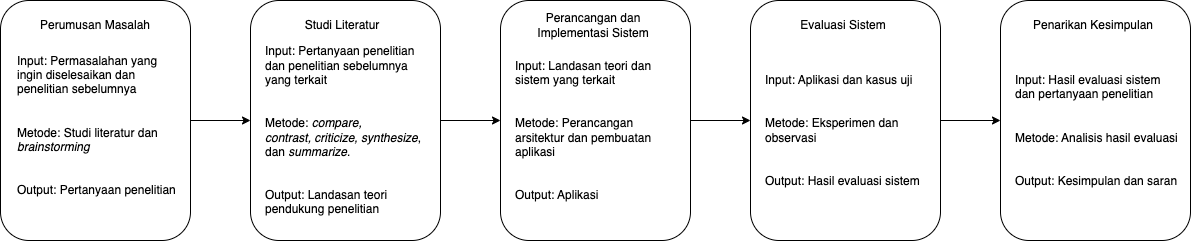
\includegraphics[width=\textwidth]{assets/pics/metode}
	\caption{Langkah penelitian.}
	\label{fig:metode}
\end{figure}

Tahapan pertama dalam penelitian ini adalah perumusan masalah. Penulis merumuskan masalah yang berasal dari permasalahan proses \textit{delivery order} pada sistem Nasional \textit{Single Window} saat ini dan literatur-literatur terkait. Kemudian dipilih satu masalah yang disorot untuk kemudian dioptimisasi. Perumusan masalah ini menghasilkan pertanyaan penelitian.

Tahapan kedua adalah studi literatur. Penulis melakukan pencarian atas penelitian terkait dengan pertanyaan penelitian. Penulis melakukan \textit{compare, contrast, criticize, synthesize, dan summarize} atas literatur-literatur terkait sehingga membentuk suatu landasan teori yang dapat menjadi pendukung penelitian. 

Tahapan ketiga adalah perancangan arsitektur, \textit{smart contract}, dan simulator. Dilakukan perancangan \textit{logic} \textit{smart contract} menggunakan Hyperledger Fabric SDK untuk proses bisnis pembuatan permohonan \textit{delivery order}. Pada tahap ini juga dirancang arsitektur untuk kebutuhan \textit{testing} atau simulasi. Kemudian dirancang simulator untuk dilakukan simulasi dan eksperimen terhadap \textit{smart contract} yang telah dibuat.

Kemudian, untuk tahapan keempat adalah evaluasi sistem. Dilakukan pengujian \textit{smart contract} dengan simulator yang telah dibuat. Hasil simulasi dan eksperimen kemudian dianalisis dan dievaluasi.

Terakhir, tahapan kelima pada penelitian ini ditarik sebuah kesimpulan dari hasil analisis dan evaluasi eksperimen. Tahapan ini menghasilkan jawaban dari pertanyaan-pertanyaan penelitian yang dirumuskan pada tahap pertama serta saran untuk penelitian selanjutnya.


\section{Metrik Evaluasi}
\label{sec:metrikevaluasi}

Pada penelitian ini, dilakukan uji dan evaluasi \textit{smart contract} menggunakan simulator yang dibuat. Skenario simulasi didasarkan pada permasalahan-permasalahan pada sistem INSW saat ini. Metode evaluasi berupa analisis \textit{log} aplikasi. Evaluasi pertama berupa analisis keamanan berdasarkan aspek \textit{security services} berupa \textit{integrity}, \textit{non-repudiation}, \textit{data confidentiality}, \textit{access control}, \textit{availability}, dan \textit{authentication}.

Evaluasi kedua adalah uji performa aplikasi. Sistem diuji dengan melakukan simulasi pembuatan \textit{delivery order} dalam waktu yang bersamaan dengan jumlah yang inkremental. Kemudian dilakukan analisis terhadap perubahan-perubahan yang terjadi saat jumlah \textit{request} ditingkatkan.

\clearchapter
%-----------------------------------------------------------------------------%
\chapter{\babEmpat}
\label{bab:4}
%-----------------------------------------------------------------------------%
Bab ini membahas desain dan implementasi sistem dalam penelitian ini. Pembahasan
dilakukan mulai dari proses permohonan ekspor dan impor barang, rancangan arsitektur sistem secara umum, rancangan infrastruktur sistem, dan rancangan arsitektur \textit{blockchain}. Dilanjutkan dengan pembahasan simulasi blockchain, dan desain evaluasi dari sistem INSW yang dikembangkan.

\section{Proses Permohonan Ekspor dan Impor Barang}
\label{sec:proses_do}
Proses permohonan dimulai dari pengguna akhir membuat permohonan melalui perusahaan eksportir dan importir. Perusahaan tersebut kemudian yang mengajukan permohonan ekspor/impor barang ke sistem INSW. Permohonan ini akan dilakukan pengecekan terhadap aturan-aturan yang ada terhadap barang-barang yang akan diekspor atau diimpor.

Proses permohonan dapat dilihat pada gambar ...

\section{Rancangan Sistem \textit{Blockchain}}
\label{sec:rancangansistem}

Komponen-komponen dalam jaringan Fabric antara lain \textit{organization}, \textit{channel}, MSP, CA, \textit{peer}, \textit{orderer} dan \textit{chaincode}. Rancangan arsitektur Fabric dijelaskan pada bagian selanjutnya.

\subsection{\textit{Channel}}
\label{subsec:channel}

\textit{Channel} merupakan grup kumpulan organisasi-organisasi dalam jaringan fabric yang terlibat pada aplikasi. \textit{Channel} dianalogikan seperti sebuah \textit{subnet} dalam jaringan, dan secara efektif berfungsi sebagai isolasi data dari organisasi lain yang bukan anggota dalam sistem ini namun masih terhubung dalam jaringan Fabric. Sistem INSW dirancang menggunakan satu \textit{channel} dengan nama "singlewindow" karena organisasi-organisasi yang terlibat akan mengakses semua data yang dirancang pada sistem ini. Konfigurasi \textit{channel} didefinisikan pada \textit{file} bernama configtx.yaml.

\subsection{Organizations}
\label{subsec:organization}

Selanjutnya dibahas komponen \textit{organization}. \textit{Organizations} merupakan representasi kelompok-kelompok yang menjadi anggota suatu \textit{channel}. Dalam kasus ini \textit{organizations} merepresentasikan perusahaan-perusahaan. Dalam penelitian ini digunakan dua 3 organisasi yaitu example.com, singlewindow.example.com, dan tradingcompany1.example.com. Setiap organisasi berkontribusi ke jaringan Fabric dengan menyumbang \textit{peer}. Organisasi example.com merupakan organisasi dalam jaringan Fabric yang bertugas menjadi \textit{orderer} untuk melaksanakan konsensus. Organisasi selanjutnya adalah singlewindow.example.com yang merepresentasikan perusahaan INSW yang bertugas sebagai administrator \textit{channel}. Singlewindow memiliki wewenang untuk mengatur, membuat, dan mengubah aturan terhadap barang ekspor dan impor. Organisasi tradingcompany1.example.com merepresentasikan perusahaan eksportir dan importir yang bergabung dalam jaringan \textit{blockchain}. Pengajuan permohonan ekspor dan impor barang dilakukan melalui organisasi ini (perusahaan eksportir dan importir). Definisi organizations dapat dilihat pada Kode \ref{lst:configtx-orgs} yang merupakan bagian dari configtx.yaml

\lstinputlisting[label={lst:configtx-orgs}, caption={Konfigurasi organisasi}]{assets/codes/configtx_organization.yaml}

\subsection{\textit{Endorsement Policy}}
\textit{Endorsement policy} adalah aturan yang perlu dicapai untuk memvalidasi sebuah transaksi. Organisasi menyetujui \textit{endorsement policy} ketika melakukan \textit{approve} pada \textit{chaincode} yang akan digunakan. Dalam penelitian ini digunakan \textit{endorsement policy} mayoritas dan didefinisikan dalam \textit{channel} agar \textit{endorsement policy} secara otomatis diperbarui ketika organisasi bergabung maupun meninggalkan \textit{channel}.

\subsection{\textit{Peer} dan \textit{Orderer}}
\label{subsec:peer-orderer}

Komponen selanjutnya yang dibahas adalah \textit{peer}. \textit{Peer} merupakan komponen penting tempat \textit{ledger} disimpan dan sebagai tempat eksekusi \textit{smart contract}. Dalam Hyperledger Fabric terdapat dua jenis \textit{peer}: \textit{orderer} dan normal. \textit{Orderer} adalah jenis \textit{peer} yang bertugas melakukan pengurutan terhadap semua \textit{event} yang terjadi pada \textit{channel}. \textit{Orderer} dalam Fabric menggunakan algoritma konsensus Raft. Sebelumnya, terdapat tiga pilihan algoritma konsensus pada \textit{orderer} yaitu Solo, untuk \textit{orderer singular}, Kafka, dan Raft. Namun, konsensus Solo dan Kafka ditandai sebagai \textit{deprecated} untuk versi 2 ke atas sehingga digunakan konsensus Raft dalam penelitian ini. Selain itu, tipe konsensus Raft sudah tersedia secara \textit{native} dalam \textit{source code orderer} sehingga tidak membutuhkan \textit{setup} ekstra seperti halnya konsensus Kafka serta penggunaan Raft memungkinkannya untuk setiap organisasi berkontribusi menjadi \textit{orderer}.

Untuk pengaturan organisasi, setiap organisasi dibuatkan satu \textit{peer} dengan rincian sebagai berikut: orderer.example.com untuk \textit{peer} orderer, peer0.singlewindow.example.com untuk \textit{peer} milik organisasi singlewindow, dan peer0.tradingcompany1.example.com untuk \textit{peer} milik organisasi tradingcompany1. Dalam rancangan ini hanya digunakan satu organisasi untuk \textit{orderer} untuk eksperimen.

Konfigurasi \textit{orderer} dapat dilihat pada Kode \ref{lst:configtx-orderers}. 

\lstinputlisting[label={lst:configtx-orderers}, caption={Konfigurasi orderer}]{assets/codes/configtx_orderer.yaml}

\subsubsection{\textit{Anchor Peer} dan \textit{Gossip Protocol}}
\label{subsubsec:anchor-peer}
Selain untuk \textit{peer} \textit{orderer}, \textit{peer} dapat dijadikan \textit{anchor peer} untuk menjadi \textit{endpoint} untuk \textit{peer} lain untuk menerapkan \textit{gossip protocol}. \textit{Anchor peer} dijadikan sebagai titik \textit{redundancy} ketika terjadi masalah koneksi antara \textit{peer} ke \textit{orderer}. \textit{Anchor peer} dan \textit{orderer} dijadikan sebagai titik komunikasi antar-\textit{peer} menggunakan \textit{gossip protocol}. \textit{Peer} peer0.singlewindow.example.com dijadikan sebagai \textit{anchor peer} dalam penelitian ini. 

\subsection{\textit{Chaincode} dan \textit{Smart Contracts}}
\label{subsec:chaincode}
Aplikasi \textit{blockchain} diimplementasikan menggunakan satu \textit{chaincode} bernama do\_chaincode dengan dua \textit{smart contract}: GoodContract dan OrderContract. \textit{GoodContract} mengatur daftar barang dan batas-batas yang diperbolehkan untuk diimpor atau diekspor. Sedangkan OrderContract berisi fungsi untuk membaca dan membuat \textit{delivery order}. \textit{Chaincode} dibuat menggunakan \textit{library} fabric-contract-api-go/contractapi. Fungsi-fungsi pada do\_chaincode yang dibuat dapat dilihat pada tabel \ref{table:smartcontract}. 

\begin{center}
\begin{table}
\begin{tabular}{ |c|c|c|c| } 
 \hline
 \textit{\textbf{Smart Contract}} & \textbf{Fungsi} & \textbf{Deskripsi} & \textbf{Pengakses} \\ 
 \hline
 GoodContract & CreateGood & Melakukan pembuatan \textit{good} (barang) & organisasi INSW \\ 
 \hline
 GoodContract & GetGoodById & Membaca \textit{good} yang ada & anggota \textit{channel} \\ 
 \hline
 OrderContract & CreateOrder & Membuat \textit{delivery order} & INSW dan perusahaan \\
 \hline
 OrderContract & ReadOrder & Membaca \textit{delivery order} & anggota \textit{channel} \\
 \hline
\end{tabular}
\caption{Tabel Fungsi \textit{Smart Contract}}
\label{table:smartcontract}
\end{table}
\end{center}

\subsection{Fabric CA Server dan Cryptogen}
\label{subsec:fabric-ca}
Fabric CA Server merupakan aplikasi CA server untuk membuat \textit{credential} berupa \textit{certificate, ca}, dan \textit{private key} untuk suatu organisasi. CA dibutuhkan Fabric sebagai identitas pada anggota \textit{blockchain} karena Fabric merupakan \textit{permissioned blockchain} yang hanya anggota tertentu yang diizinkan untuk bergabung ke jaringan. Untuk kebutuhan \textit{testing}, terdapat \textit{tool} bernama Cryptogen untuk membuat semua \textit{credential} yang dibutuhkan untuk tiap organisasi yang didefinisikan melalui suatu \textit{file config}. Dalam penelitian ini tidak digunakan Fabric CA Server melainkan menggunakan Cryptogen sebagai pembuat identitas karena hanya digunakan untuk keperluan simulasi, tidak untuk lingkungan \textit{production}. \textit{Config} Cryptogen untuk membuat identitas dapat dilihat pada \textit{file} \ref{lst:cryptogen} 

\lstinputlisting[label={lst:cryptogen}, caption={Konfigurasi cryptogen}]{assets/codes/cryptogen.yaml}

\subsection{\textit{Deployment}}
\label{subsec:deployment}
Infrastruktur \textit{blockchain} di-\textit{deploy} menggunakan Docker pada \textit{host machine} Apple Macbook Pro 2021 dengan \textit{chip} Apple M1 Pro dan \textit{Memory} 16 Gb. \textit{File compose} untuk \textit{deployment} Fabric dapat dilihat pada \textit{file} \ref{lst:compose}.

\lstinputlisting[label={lst:compose}, caption={Konfigurasi \textit{compose}}]{assets/codes/compose.yaml}

\section{Rancangan Simulasi}
\label{sec:simulation}
Pengujian sistem dan \textit{smart contract} dilakukan dengan sebuah simulator. Simulator dirancang sebagai program untuk memanggil \textit{smart contract} yang dibuat. Simulator dibuat dalam bahasa pemrograman Go menggunakan \textit{library} fabric-gateway/pkg/client dan grpc. Rincian kasus uji simulator adalah sebagai berikut.

\subsection{Inisialisasi \textit{Fabric Gateway Client}}
Untuk berkomunikasi dengan jaringan \textit{fabric} perlu dilakukan inisialisasi \textit{client} terlebih dahulu. Pertama program perlu menginisiasi koneksi \textit{gRPC} ke \textit{peer} dengan menyertakan sertifikat TLS, kemudian membuat \textit{identity} dan \textit{sign}. Selanjutnya membuat sebuah \textit{gateway connection} yang disediakan oleh \textit{library} fabric-gateway/pkg/client di atas koneksi \textit{gRPC} yang telah dibuat dengan menyertakan \textit{evaluate timeout, endorse timeout, submit timeout,} dan \textit{commit timeout}. Langkah terakhir adalah mengambil objek \textit{smart contract} dari \textit{gateway connection} yang telah dibuat dengan memanggil metode \textbf{GetContractWithName()} dengan parameter nama \textit{chaincode} dan nama \textit{smart contract}, yang dalam kasus ini perlu mengambil dua objek \textit{smart contract} GoodContract dan OrderContract. 

Terdapat dua cara untuk memanggil fungsi pada \textit{smart contract} yaitu memanggil metode \textbf{SubmitTransaction()} dan \textbf{EvaluateTransaction()}. \textbf{SubmitTransaction()} digunakan untuk melakukan operasi yang mengubah data dalam \textit{world state} (\textit{unsafe operation}) dan transaksi dicatat dalam blok. Sedangkan metode \textbf{EvaluateTransaction()} digunakan untuk membaca data dari \textit{world state} yang telah ter-commit (\textit{safe operation} dan pemanggilan \textit{chaincode} hanya dilakukan secara lokal sehingga tidak melibatkan \textit{peer} lain dan \textit{orderer}.

Ketika metode \textbf{SubmitTransaction()} dipanggil, Pemanggilan fungsi dipropagasi ke semua \textit{endorsing peer} untuk dieksekusi \textit{chaincodenya} pada masing-masing \textit{endorsing peer}. Setelah mencapai kesepakatan (tidak terbatas pada mayoritas, diatur saat pengaturan \textit{channel}), transaksi dikirim ke \textit{orderer} untuk dibuatkan blok. Setelah blok dibuat blok akan dikirim ke semua \textit{peer}.

Untuk kasus uji simulasi \textit{request} \textit{concurrent}, akan diuji dengan \textit{client} yang diatur dengan \textit{timeout} dan tanpa \textit{timeout}. Durasi \textit{timeout} yang digunakan adalah angka \textit{default} dari \textit{repo} fabric-samples.

\subsection{Inisialisasi Barang}
\label{subsec:init-good}
Simulasi dimulai dengan membuat daftar barang yang diperbolehkan untuk ekspor maupun impor. Sepuluh barang dibuat dengan memanggil fungsi CreateGood dari \textit{smart contract} GoodContract sebanyak sepuluh kali. \textit{Field} \textit{unit, importLimit}, dan \textit{exportLimit} dibuat serupa untuk mensimplifikasi inisialisasi barang. Langkah inisialisasi dapat dilihat pada potongan kode \ref{lst:initgood}.

\lstinputlisting[label={lst:initgood}, caption={Inisialisasi \textit{Good}}]{assets/codes/initgood.go}

Untuk melihat data barang yang telah dibuat, simulator mengambil data barang yang telah dibuat pada \ref{subsec:init-good} dengan memanggil fungsi \textit{chaincode} \textbf{GetGoodById()}. Simulasi membaca barang dapat dilihat pada fungsi \ref{lst:readgood}.

\lstinputlisting[label={lst:readgood}, caption={Membaca \textit{good} yang telah dibuat}]{assets/codes/readgood.go}

\subsection{Membuat \textit{Order}}
Setelah daftar barang dibuat, simulasi selanjutnya adalah membuat \textit{order}. \textit{Order} dibuat menggunakan identitas tradingcompany1 untuk mensimulasi sebuah perusahaan yang membuat \textit{delivery order}. Terdapat dua kasus dalam membuat \textit{order}. Yang pertama adalah pembuatan \textit{order} dengan barang yang memenuhi syarat batas impor atau ekspor. Kasus kedua adalah pembuatan \textit{order} dengan barang yang melebihi batas impor atau ekspor. Simulasi pembuatan \textit{order} yang memenuhi syarat terhadap daftar barang yang dikirim dapat dilihat pada fungsi \ref{lst:createorder}. Sedangkan simulasi pembuatan \textit{order} dengan barang yang melebihi kapasitas dapat dilihat pada fungsi \ref{lst:createorderlimit}. Setelah \textit{order} dibuat, simulator membaca \textit{order} dengan kode \ref{lst:readorder} berikut.

\lstinputlisting[label={lst:createorder}, caption={Membuat \textit{order} sesuai dengan aturan barang}]{assets/codes/createorder.go}

\lstinputlisting[label={lst:createorderlimit}, caption={Membuat \textit{order} dengan barang yang melebihi batas}]{assets/codes/createorderlimit.go}

\lstinputlisting[label={lst:readorder}, caption={Membaca \textit{order}}]{assets/codes/readorder.go}


\subsection{Membuat Barang Dengan Identitas Yang Tidak Terotorisasi}
Kasus simulasi selanjutnya adalah mencoba membuat barang menggunakan identitas selain milik organisasi singlewindow.example.com. Kasus ini dimaksudkan untuk menguji \textit{access control} pada \textit{smart contract} GoodContract. Simulasi kasus ini dapat dilihat pada fungsi \ref{lst:creategoodunauthorized}.

\lstinputlisting[label={lst:creategoodunauthorized}, caption={Membuat \textit{good} menggunakan identitas yang tidak terotorisasi}]{assets/codes/creategoodunauthorized.go}

\subsection{Membuat \textit{Order} secara bersamaan}
Selanjutnya, untuk menguji \textit{performance} dan mencari \textit{upper bound} dari \textit{request} yang bersamaan, simulator melakukan pembuatan \textit{order} secara \textit{concurrent}. Pengujian ini dilakukan dengan dua konfigurasi \textit{client} yang berbeda. Yang pertama adalah konfigurasi \textit{client} tanpa batas waktu \textit{timeout} untuk menguji ketahanan sistem dalam melayani \textit{request}. Konfigurasi yang kedua adalah konfigurasi \textit{client} dengan \textit{timeout} berikut: \textit{evaluate timeout} 5 detik, \textit{endorse timeout} 15 detik, \textit{submit timeout} 5 detik, dan \textit{commit timeout} 1 menit. Angka tersebut merupakan angka yang diambil dari konfigurasi \textit{client} pada \textit{repo} fabric-samples. Untuk kasus uji dengan \textit{timeout}, jumlah \textit{request} ditingkatkan secara inkremental yaitu 9, 10, 100, 1000, 2000, 3000, 4000, 5000, 6000, 7000, 8000, 9000, dan 10000. Sedangkan untuk kasus tanpa \textit{timeout}, jumlah \textit{request} secara meningkat adalah 9, 10, 100, 1000, 10000, dan 100000. Untuk setiap iterasi dicatat waktu eksekusi dan jumlah transaksi yang gagal. Simulasi untuk kasus ini dapat dilihat pada fungsi \ref{lst:concurrentorder}.

\lstinputlisting[label={lst:concurrentorder}, caption={Membuat \textit{order} secara bersamaan}]{assets/codes/concurrentorder.go}







\clearchapter
%-----------------------------------------------------------------------------%
\chapter{\babLima}
\label{bab:5}
%-----------------------------------------------------------------------------%
Pada bab ini dijelaskan hasil eksperimen yang dilakukan pada skenario simulasi pada subbab \ref{sec:simulation}. Dilakukan pembahasan dan analisis terhadap hasil pengujian berdasarkan skenario dan dihubungkan dengan aspek \textit{authentication, access control, availability} dan performa.

\section{Hasil dan Analisis Fungsional \textit{Smart Contract}}
Pada bagian ini dibahas hasil simulasi yang dilakukan pada subbab \ref{sec:simulation}. 

\subsection{Pembuatan Barang}
\label{subsec:creategood-chap5}
Hasil simulasi pembuatan barang dapat dilihat pada log \ref{lst:creategoodlog}. Pembuatan barang dilakukan pada tahap inisialisasi barang dan log diambil pada 2 barang pertama. Dapat dilihat pada log untuk setiap barang yang dibuat transaksi dicatat dalam \textit{block} dan memakan waktu 2 detik hingga transaksi ter-\textit{commit} dalam block. Hal ini dikarenakan dalam simulator, \textit{client} melakukan SubmitTransaction untuk membuat barang dipanggil secara sinkronus dan menunggu hasil hingga transaksi ter-\textit{commit} dalam \textit{block}. 

\lstinputlisting[label={lst:creategoodlog}, caption=Log pembuatan barang]{assets/logs/8_CreateGood.txt}

Dapat dilihat bahwa untuk setiap pemanggilan SubmitTransaction, transaksi dipropagasi ke seluruh \textit{peer} yang terhubung dan tergabung dalam \textit{channel} singlewindow kemudian \textit{chaincode} dieksekusi pada setiap \textit{peer} untuk dilakukan \textit{endorse} transaksi. Hal ini dapat dilihat pada log peer0.tradingcompany1.example.com pada indeks \textbf{adcc} dan \textbf{add1}. Setelah mayoritas \textit{peer} selesai melakukan \textit{endorse}, transaksi dikirim ke \textit{orderer} untuk kemudian dilakukan \textit{event ordering} dan dibuatkan \textit{block}. Setelah \textit{block} selesai dibuat \textit{block} disebarkan ke seluruh peer anggota jaringan dan kemudian di-commit pada masing-masing \textit{peer}. Kemudian dapat dilihat untuk \textit{block} yang telah dibuat (\textit{block} 711 dan 712) memiliki nilai \textit{hash} yang sama di setiap \textit{peer}.

\subsection{Membaca Barang}
\label{subsec:readgoodlog}
Untuk melihat barang yang telah ditambah sebelumnya, dilakukan pembacaan barang. Hasil dari simulasi ini dapat dilihat pada log \ref{lst:readgoodlog}. Untuk membaca data dari \textit{world state}, digunakan \textit{API} EvaluateTransaction. Berbeda dengan SubmitTransaction, pemanggilan ini bersifat lokal dan hanya membaca melalui \textit{peer} yang dituju. Dapat dilihat bahwa hanya \textit{peer} peer0.singlewindow.example.com yang menerima transaksi EvaluateTransaction dan tidak dikirim ke \textit{orderer} sehingga tidak ada \textit{block} yang dibuat.

\lstinputlisting[label={lst:readgoodlog}, caption=Log pembacaan barang]{assets/logs/9_ReadGood.txt}

\subsection{Membuat \textit{Order}}
Setelah daftar barang dipastikan ada, dilakukan pembuatan dua \textit{order}. \textit{Order} pertama adalah \textit{order} dengan spesifikasi barang yang tidak melebihi batas impor maupun ekspor. Hasil pembuatan \textit{order} dapat dilihat pada log \ref{lst:createorderlog}. Terdapat log pada \textit{chaincode} yang menunjukkan alur pembuatan \textit{order}. Untuk log pada \textit{peer} dan \textit{orderer} serupa dengan log pada subbab \ref{subsec:creategood-chap5} yaitu pemanggilan \textit{chaincode}, \textit{endorse}, \textit{submit} transaksi ke \textit{orderer}, kemudian \textit{commit}. 

\lstinputlisting[label={lst:createorderlog}, caption=Log pembuatan \textit{order}]{assets/logs/10_CreateOrderSuccess.txt}

Pembuatan \textit{order} yang kedua adalah pembuatan \textit{order} dengan kuantitas barang yang melebihi batas yang diperbolehkan. Hasil pengujian berupa log yang dapat dilihat pada log \ref{lst:createorderfailedlog}. Pada log \textit{chaincode} dapat dilihat bahwa pembuatan gagal pada saat melakukan verifikasi terhadap kuantitas barang yang terhadap aturan pada barang tersebut. Karena transaksi tersebut mengembalikan \textit{error} transaksi tersebut tidak disebarkan ke \textit{peer} lain sehingga tidak di-endorse dan tidak dikirim ke \textit{orderer}.

\lstinputlisting[label={lst:createorderfailedlog}, caption=Log pembuatan \textit{order} yang gagal]{assets/logs/12_CreateInvalidOrder.txt}

\subsection{Membaca \textit{Order}}
Untuk memasikan \textit{order} telah berhasil dibuat dilakukan pengujian dengan membaca \textit{order} yang sebelumnya dibuat. Hasil pembacaan \textit{order} dapat dilihat pada log \ref{lst:readorderlog}. Seperti halnya pada saat membaca barang pada subbab \ref{subsec:readgoodlog} yaitu menggunakan \textit{api} EvaluateTransaction() dan \textit{chaincode} dieksekusi hanya secara lokal (tidak melibatkan \textit{peer} lain.)

\lstinputlisting[label={lst:readorderlog}, caption=Log pembacaan \textit{order}]{assets/logs/11_ReadCreatedOrder.txt}

\section{Hasil dan Analisis Aspek \textit{Authentication}}
Untuk melakukan analisis terhadap aspek \textit{authentication}, dilakukan pengujian dengan cara mengakses aplikasi dengan identitas dan \textit{peer} yang berbeda. Hyperledger Fabric mengharuskan untuk organisasi untuk berkomunikasi dengan \textit{blockchain} melalui \textit{peer} milik organisasi tersebut. Uji otentikasi dilakukan dengan mengatur \textit{credential client}  menggunakan identitas organisasi tradingcompany1.example.com untuk melakukan koneksi melalui \textit{peer} milik organisasi singlewindow.example.com. Dapat dilihat pada log \ref{lst:differentpeer} bahwa \textit{client} tidak terotorisasi dan ditolak untuk berkomunikasi melalui \textit{peer} milik organisasi singlewindow.example.com

\lstinputlisting[label={lst:differentpeer}, caption=\textit{Request} menggunakan \textit{peer} organisasi lain]{assets/logs/16_SubmitToOtherOrganizationPeer.txt}

\section{Hasil dan Analisis Aspek \textit{Access Control}}
Selanjutnya, untuk menguji aspek \textit{access control}, dilakukan pemanggilan fungsi CreateGood() yang telah didefinisikan pada tabel \ref{table:smartcontract} menggunakan identitas milik organisasi tradingcompany.example.com, yang seharusnya hanya dapat dipanggil oleh organisasi singlewindow.example.com. Hasil pengujian ini dapat dilihat pada log \ref{lst:creategoodunauthorizedlog}. Dapat dilihat pada log bahwa pemanggilan \textit{chaincode} gagal dan mengembalikan \textit{error} sehingga INSW tetap dapat mengatur barang-barang yang diperbolehkan tanpa diubah oleh pihak tidak berwenang.

\lstinputlisting[label={lst:creategoodunauthorizedlog}, caption=Membuat barang menggunakan identitas tidak terotorisasi]{assets/logs/13_CreateGoodUnauthorized.txt}

\section{Hasil dan Analisis Aspek Performa dan \textit{Availability}}
Selanjutnya, aspek performa dan \textit{availability} diuji dengan mengirim \textit{request} secara \textit{concurrent}. Hasil pengujian untuk \textit{request concurrent} tanpa timeout dapat dilihat pada log \ref{lst:concurrentnotimeout}. Dapat dilihat bahwa sistem tetap mampu melayani \textit{request} hingga 10000 namun terjadi \textit{crash} saat melayani 100000 \textit{request}. 

\lstinputlisting[label={lst:concurrentnotimeout}, caption=\textit{Request concurrent} tanpa \textit{timeout client}]{assets/logs/14_ConcurrentOrderNoTimeout.txt}

Sedangkan untuk hasil uji \textit{request concurrent} dengan \textit{timeout} pada \textit{client} dapat dilihat pada log \ref{lst:concurrentwithtimeout}. Dalam 5 iterasi, 4 dari 5 iterasi mengalami kegagalan pada 4000 \textit{request} ke atas dan 1 dari 5 iterasi terdapat 8 \textit{request} gagal pada 3000 \textit{request}. Untuk durasi 9 request adalah sekitar 2 detik sedangkan untuk \textit{request} hanya berdurasi rata-rata 0.14 detik. Hal ini dikarenakan dalam konfigurasi \textit{orderer}, \textit{block} akan menampung transaksi dalam \textit{batch} 10 transaksi setiap \textit{block} dengan \textit{timeout} 2 detik. Dengan kata lain pembuatan \textit{block} akan ditunda hingga 2 detik jika jumlah transaksi kurang dari 10.

\lstinputlisting[label={lst:concurrentwithtimeout}, caption=\textit{Request concurrent} dengan \textit{timeout client}]{assets/logs/15_ConcurrentOrderWithNormalTimeout.txt}

\subsection{Potensi Serangan \textit{Denial-of-Service}}
Jika dibandingkan antara dua skenario untuk \textit{client} dengan \textit{timeout} dan tanpa \textit{timeout}, \textit{client} dengan timeout akan menggagalkan \textit{request} yang sedang berlangsung jika menunggu terlalu lama untuk menyelesaikan tahap-tahapan transaksi. Namun ketika \textit{client} dikonfigurasi tanpa menggunakan \textit{timeout}, sistem tetap akan melayani \textit{request} hingga selesai dibuatkan \textit{block} sehingga untuk melakukan transaksi baru harus menunggu seluruh transaksi sebelumnya selesai diproses. Hal ini menimbulkan celah serangan yang membuat sistem mengalami \textit{denial-of-service} dengan cara melakukan \textit{spam request} dengan jumlah yang sangat banyak. Untuk mengatasi hal ini dapat diterapkan \textit{rate limiting} untuk setiap \textit{client} yang menggunakan sistem ini.

\clearchapter
\include{src/01-body/bab6}
\clearchapter
%---------------------------------------------------------------
\chapter{\kesimpulan}
\label{bab:6}
%---------------------------------------------------------------
Pada bab ini, dijelaskan kesimpulan atas penelitian sistem \textit{delivery order} berbasis \textit{blockchain} Hyperledger Fabric. Terdapat juga saran untuk pengembang dan serta saran untuk penelitian selanjutnya.


%---------------------------------------------------------------
\section{Kesimpulan}
\label{sec:kesimpulan}
%---------------------------------------------------------------

Proses verifikasi manual pada pembuatan \textit{delivery order} dapat dihilangkan. Proses tersebut dapat diimplementasi menggunakan komponen \textit{chaincode} pada Hyperledger Fabric. Dengan adanya \textit{smart contract} yang menggantikan proses manual, kegiatan penyelewengan seperti penyuapan dapat menurun karena semakin sedikit celah untuk dapat dilakukan intervensi. 

Untuk mengimplementasi \textit{chaincode} digunakan \textit{library} fabric-contract-api sedangkan untuk mengaksesnya dibutuhkan suatu \textit{frontend} dan \textit{client} yang dapat diimplementasi menggunakan \textit{library} fabric-gateway. \textit{Library fabric-contract-api} memiliki antarmuka fungsi untuk membaca dan menyimpan data dari dan ke \textit{ledger}. Fitur membaca data pada \textit{library} ini (GetState()) dimanfaatkan pada logika pembuatan \textit{delivery order} pada \textit{smart contract} untuk verifikasi daftar barang yang akan dikirim.

Sementara untuk cara mengimplementasi proses \textit{delivery order} menggunakan bantuan Hyperledger Fabric SDK adalah, melengkapi yang telah disebutkan di paragraf sebelumnya, dengan membuat dua tipe penyimpanan data yaitu data barang dan data \textit{delivery order}. Verifikasi daftar barang yang akan dikirim dalam \textit{delivery order} dilakukan dengan membaca data barang-barang menggunakan fungsi GetState() untuk diverifikasi batasnya dengan kuantitas yang ingin dikirim. Setelah semua terverifikasi dan sah, data \textit{delivery order} disimpan ke \textit{ledger} dengan fungsi PutState() kemudian ditunggu hingga \textit{block} untuk transaksi tersebut sudah dibuat dan transaksi sudah di-\textit{commit}. Data \textit{order} yang telah di-\textit{commit} tersebut menandakan bahwa \textit{delivery order} telah berhasil dan selesai dibuat.

Keunggulan lain sistem \textit{delivery order} berbasis \textit{blockchain} dalam aspek \textit{authentication} yaitu sistem hanya dapat diakses oleh pihak yang sudah terdaftar dalam jaringan \textit{blockchain} sehingga sistem tidak dapat diakses oleh pihak tidak dikenal. Untuk aspek \textit{access control}, fitur tertentu masih dapat dibatasi hanya dapat diakses oleh organisasi tertentu, yang dalam hal ini pengaturan dan pengubahan tentang daftar barang untuk dikirim hanya dapat dilakukan oleh pihak INSW. Kemudian untuk aspek \textit{reliability} menurut eksperimen sistem dapat melayani hingga 2000 \textit{request} bersamaan tanpa terdapat transaksi yang gagal.

Melihat kembali pada celah potensi penyuapan pada sistem INSW saat ini, celah tersebut dapat dihilangkan dengan mengganti proses verifikasi manual menjadi bagian dari \textit{logic smart contract}. Solusi tersebut dapat juga diimplementasikan menggunakan sistem tradisional yang tersentralisasi dan menggunakan \textit{database}. Namun dikarenakan banyak organisasi luar yang akan menggunakan sistem ini, diperlukan tingkat transparansi serta keamanan yang lebih tinggi untuk meningkatkan kepercayaan pengguna sistem. Dalam hal ini pendekatan \textit{blockchain} memiliki keunggulan dalam hal transparansi dan keamanan dari karakteristik \textit{tamper-evident} dan \textit{tamper-resistant} (lihat Subbab \ref{sec:litblockchain}) pada \textit{blockchain} yang tidak dimiliki oleh sistem tradisional.

%---------------------------------------------------------------
\section{Saran}
\label{sec:saran}
%---------------------------------------------------------------
Berdasarkan hasil penelitian ini, terdapat saran untuk pengembang dan untuk penelitian selanjutnya. Dikarenakan sistem memiliki celah serangan \textit{spam} yang dapat mengakibatkan sistem \textit{denial-of-service}, saran pertama yaitu perlu diimplementasikannya \textit{rate limiting} untuk membatasi jumlah \textit{request} yang bisa diajukan oleh \textit{client}. Selain itu dapat juga diimplementasikan \textit{cryptocurrency} sebagai biaya transaksi . Saran kedua yaitu dapat dilakukan penelitian lebih lanjut untuk aspek efisiensi, \textit{scalability}, \textit{latency}, dan aspek lainnya.

Teknologi \textit{blockchain} masih memiliki potensi-potensi lain dalam sistem \textit{supply-chain} maupun sistem-sistem lainnya. Ditambah dengan meningkatnya \textit{trend} dan publikasi penelitian aplikasi \textit{blockchain} \citep{Macrinici2018} semakin mendekatnya teknologi \textit{blockchain} dapat diadaptasi lebih banyak. Penelitian ini diharapkan dapat membantu bagi pengembang aplikasi \textit{blockchain} maupun membantu untuk penelitian-penelitian \textit{blockchain} setelah ini.

\clearchapter

%
% Daftar Pustaka
\CAPinToC % All entries in ToC will be CAPITALIZED from here on
\include{_internals/pustaka}
\clearchapter
\noCAPinToC % Revert to original \addcontentsline formatting

%
% Lampiran
%
\begin{appendix}
	\newcounter{pagetemp}
	\setcounter{pagetemp}{\thepage}
	\include{_internals/markLampiran}
	\clearchapter
	\setcounter{page}{\thepagetemp}
	\stepcounter{page}
	%-----------------------------------------------------------------------------%
\addappendix{CHANGELOG}
\chapter*{Lampiran 1: CHANGELOG}
\label{appendix:changelog}
%-----------------------------------------------------------------------------%


%-----------------------------------------------------------------------------%
\addappendix{Judul Lampiran 2}
\chapter*{Lampiran 2: Judul Lampiran 2}
\label{appendix:sample}
%-----------------------------------------------------------------------------%
Lampiran hadir untuk menampung hal-hal yang dapat menunjang pemahaman terkait tugas akhir, namun akan mengganggu \f{flow} bacaan sekiranya dimasukkan ke dalam bacaan.
Lampiran bisa saja berisi data-data tambahan, analisis tambahan, penjelasan istilah, tahapan-tahapan antara yang bukan menjadi fokus utama, atau pranala menuju halaman luar yang penting.

%-----------------------------------------------------------------------------%
\section*{Subbab dari Lampiran 2}
\label{appendix:sampleSubchap}
%-----------------------------------------------------------------------------%
\todo{Isi subbab ini sesuai keperluan Anda. Anda bisa membuat lebih dari satu judul lampiran, dan tentunya lebih dari satu subbab.}

\end{appendix}

\end{document}
